% Options for packages loaded elsewhere
\PassOptionsToPackage{unicode}{hyperref}
\PassOptionsToPackage{hyphens}{url}
\PassOptionsToPackage{dvipsnames,svgnames,x11names}{xcolor}
%
\documentclass[
  letterpaper,
  DIV=11,
  numbers=noendperiod]{scrartcl}

\usepackage{amsmath,amssymb}
\usepackage{iftex}
\ifPDFTeX
  \usepackage[T1]{fontenc}
  \usepackage[utf8]{inputenc}
  \usepackage{textcomp} % provide euro and other symbols
\else % if luatex or xetex
  \usepackage{unicode-math}
  \defaultfontfeatures{Scale=MatchLowercase}
  \defaultfontfeatures[\rmfamily]{Ligatures=TeX,Scale=1}
\fi
\usepackage{lmodern}
\ifPDFTeX\else  
    % xetex/luatex font selection
\fi
% Use upquote if available, for straight quotes in verbatim environments
\IfFileExists{upquote.sty}{\usepackage{upquote}}{}
\IfFileExists{microtype.sty}{% use microtype if available
  \usepackage[]{microtype}
  \UseMicrotypeSet[protrusion]{basicmath} % disable protrusion for tt fonts
}{}
\makeatletter
\@ifundefined{KOMAClassName}{% if non-KOMA class
  \IfFileExists{parskip.sty}{%
    \usepackage{parskip}
  }{% else
    \setlength{\parindent}{0pt}
    \setlength{\parskip}{6pt plus 2pt minus 1pt}}
}{% if KOMA class
  \KOMAoptions{parskip=half}}
\makeatother
\usepackage{xcolor}
\setlength{\emergencystretch}{3em} % prevent overfull lines
\setcounter{secnumdepth}{-\maxdimen} % remove section numbering
% Make \paragraph and \subparagraph free-standing
\makeatletter
\ifx\paragraph\undefined\else
  \let\oldparagraph\paragraph
  \renewcommand{\paragraph}{
    \@ifstar
      \xxxParagraphStar
      \xxxParagraphNoStar
  }
  \newcommand{\xxxParagraphStar}[1]{\oldparagraph*{#1}\mbox{}}
  \newcommand{\xxxParagraphNoStar}[1]{\oldparagraph{#1}\mbox{}}
\fi
\ifx\subparagraph\undefined\else
  \let\oldsubparagraph\subparagraph
  \renewcommand{\subparagraph}{
    \@ifstar
      \xxxSubParagraphStar
      \xxxSubParagraphNoStar
  }
  \newcommand{\xxxSubParagraphStar}[1]{\oldsubparagraph*{#1}\mbox{}}
  \newcommand{\xxxSubParagraphNoStar}[1]{\oldsubparagraph{#1}\mbox{}}
\fi
\makeatother


\providecommand{\tightlist}{%
  \setlength{\itemsep}{0pt}\setlength{\parskip}{0pt}}\usepackage{longtable,booktabs,array}
\usepackage{calc} % for calculating minipage widths
% Correct order of tables after \paragraph or \subparagraph
\usepackage{etoolbox}
\makeatletter
\patchcmd\longtable{\par}{\if@noskipsec\mbox{}\fi\par}{}{}
\makeatother
% Allow footnotes in longtable head/foot
\IfFileExists{footnotehyper.sty}{\usepackage{footnotehyper}}{\usepackage{footnote}}
\makesavenoteenv{longtable}
\usepackage{graphicx}
\makeatletter
\def\maxwidth{\ifdim\Gin@nat@width>\linewidth\linewidth\else\Gin@nat@width\fi}
\def\maxheight{\ifdim\Gin@nat@height>\textheight\textheight\else\Gin@nat@height\fi}
\makeatother
% Scale images if necessary, so that they will not overflow the page
% margins by default, and it is still possible to overwrite the defaults
% using explicit options in \includegraphics[width, height, ...]{}
\setkeys{Gin}{width=\maxwidth,height=\maxheight,keepaspectratio}
% Set default figure placement to htbp
\makeatletter
\def\fps@figure{htbp}
\makeatother
% definitions for citeproc citations
\NewDocumentCommand\citeproctext{}{}
\NewDocumentCommand\citeproc{mm}{%
  \begingroup\def\citeproctext{#2}\cite{#1}\endgroup}
\makeatletter
 % allow citations to break across lines
 \let\@cite@ofmt\@firstofone
 % avoid brackets around text for \cite:
 \def\@biblabel#1{}
 \def\@cite#1#2{{#1\if@tempswa , #2\fi}}
\makeatother
\newlength{\cslhangindent}
\setlength{\cslhangindent}{1.5em}
\newlength{\csllabelwidth}
\setlength{\csllabelwidth}{3em}
\newenvironment{CSLReferences}[2] % #1 hanging-indent, #2 entry-spacing
 {\begin{list}{}{%
  \setlength{\itemindent}{0pt}
  \setlength{\leftmargin}{0pt}
  \setlength{\parsep}{0pt}
  % turn on hanging indent if param 1 is 1
  \ifodd #1
   \setlength{\leftmargin}{\cslhangindent}
   \setlength{\itemindent}{-1\cslhangindent}
  \fi
  % set entry spacing
  \setlength{\itemsep}{#2\baselineskip}}}
 {\end{list}}
\usepackage{calc}
\newcommand{\CSLBlock}[1]{\hfill\break\parbox[t]{\linewidth}{\strut\ignorespaces#1\strut}}
\newcommand{\CSLLeftMargin}[1]{\parbox[t]{\csllabelwidth}{\strut#1\strut}}
\newcommand{\CSLRightInline}[1]{\parbox[t]{\linewidth - \csllabelwidth}{\strut#1\strut}}
\newcommand{\CSLIndent}[1]{\hspace{\cslhangindent}#1}

\KOMAoption{captions}{tableheading}
\makeatletter
\@ifpackageloaded{caption}{}{\usepackage{caption}}
\AtBeginDocument{%
\ifdefined\contentsname
  \renewcommand*\contentsname{Table of contents}
\else
  \newcommand\contentsname{Table of contents}
\fi
\ifdefined\listfigurename
  \renewcommand*\listfigurename{List of Figures}
\else
  \newcommand\listfigurename{List of Figures}
\fi
\ifdefined\listtablename
  \renewcommand*\listtablename{List of Tables}
\else
  \newcommand\listtablename{List of Tables}
\fi
\ifdefined\figurename
  \renewcommand*\figurename{Figure}
\else
  \newcommand\figurename{Figure}
\fi
\ifdefined\tablename
  \renewcommand*\tablename{Table}
\else
  \newcommand\tablename{Table}
\fi
}
\@ifpackageloaded{float}{}{\usepackage{float}}
\floatstyle{ruled}
\@ifundefined{c@chapter}{\newfloat{codelisting}{h}{lop}}{\newfloat{codelisting}{h}{lop}[chapter]}
\floatname{codelisting}{Listing}
\newcommand*\listoflistings{\listof{codelisting}{List of Listings}}
\makeatother
\makeatletter
\makeatother
\makeatletter
\@ifpackageloaded{caption}{}{\usepackage{caption}}
\@ifpackageloaded{subcaption}{}{\usepackage{subcaption}}
\makeatother

\ifLuaTeX
  \usepackage{selnolig}  % disable illegal ligatures
\fi
\usepackage{bookmark}

\IfFileExists{xurl.sty}{\usepackage{xurl}}{} % add URL line breaks if available
\urlstyle{same} % disable monospaced font for URLs
\hypersetup{
  pdftitle={Paper Review},
  colorlinks=true,
  linkcolor={blue},
  filecolor={Maroon},
  citecolor={Blue},
  urlcolor={Blue},
  pdfcreator={LaTeX via pandoc}}


\title{Paper Review}
\author{Shauna Heron}
\date{}

\begin{document}
\maketitle

\renewcommand*\contentsname{Table of contents}
{
\hypersetup{linkcolor=}
\setcounter{tocdepth}{3}
\tableofcontents
}

\textsubscript{Source:
\href{https://shaunaheron2.github.io/ML_Assignment2/index.qmd.html}{Article
Notebook}}

\section{\texorpdfstring{\textbf{Introduction and
Motivation}}{Introduction and Motivation}}\label{introduction-and-motivation}

This review analyzes the study by Garriga et al.~(2023), published in
\emph{Cell Medical}, titled \emph{``Combining Clinical Notes with
Structured Electronic Health Records Enhances the Prediction of Mental
Health Crises.''}

The research investigates the utility of combining unstructured clinical
notes with structured data from electronic mental health records (EMHR)
to improve the prediction of mental health crises. The relevance of
Garriga et al. (2023) study is underscored by an alarming rise in mental
health-related hospitalizations coinciding with significant resource and
workforce challenges. Recent data highlights that hospitalizations for
mental health conditions, particularly among youth in Ontario, have
surged since the COVID-19 pandemic. Mental health crises requiring
hospitalization (e.g., emotional breakdowns, substance overdoses and
suicide attempts) have increased \_\_-fold. What's worse, many of these
crises might have been prevented with early intervention. However a lack
of predictive tools has made it difficult for healthcare systems to
anticipate and address these crises before they peak.

Leveraging Electronic Health Records (EHRs) to bolster clinical
decision-making is not new, as clinicians and researchers have long
utilized structured data like diagnosis codes, lab results, and
medication records, to inform predictive models and treatment
strategies. However, due to computational restraints and \ldots. ,
unstructured data like clinical notes and other free-form text and
imagery until recently has been left largely untapped. Considering this
form of data constitutes a substantial portion of EHRs in terms of
volume and contains critical narrative information like clinician
observations, patient-reported symptoms, and contextual details
surrounding patient interactions that structured data might lack, by
incorporating this textual data into predictive models\ldots..

\subsection{Problem Statement}\label{problem-statement}

The primary objective of the study was to predict mental health crises
utilizing both structured and unstructured mental health data.

When a patient is admitted to acute care with a mental crisis it might
be their first visit or the most recent in a long history of crisis
events. At each event, a mix of information is collected including
structured data comprised of discrete variables (i.e., gender,
diagnoses, and school district), continuous variables (i.e.,
standardized assessment scores) and administrative data (i.e., number of
visits, hours of service) and time based data like intake, discharge and
assessment dates.

The main challenge posed by these data was the clinical reality that the
information contained in any one EHR varied significantly from patient
to patient. Moreover, clincian-level idosyncricies like personal style,
work habits and clinical modality meant that the quality, availability
and volume of clinical notes in EHRs was highly inconsistent. Moreover,
the severity and frequency of a patients mental health crises was
related to the volume of notes within the EHR, meaning that those with
more severe or recurrent episodes typically had a greater volume of
clinical notes. As such, it was important that to establish the minimum
quantity of unstructured data that would contribute to the accurate
prediction of mental health crises and still remain effective across a
spectrum of patient complexity, regardless of the volume of clinical
notes.

How would they contend with this probleM?

\subsection{\texorpdfstring{\textbf{Solution}}{Solution}}\label{solution}

The study extended Garriga et al. (2023) previous work that had analyzed
60,000 de-identified patient records collected over eight years to
predict mental health crisis within the next 28 days following a weekly
algorithm prediction. Their main objectives were to i) compare the
predictive power of unstructured data alone with structured data; ii)
improve performance by comparing methods for combining structured and
unstructured data; and iii) investigate the minimum amount of
unstructured data necessary to improve model accuracy.

\subsection{\texorpdfstring{\textbf{Experimental
Setup}}{Experimental Setup}}\label{experimental-setup}

To this end researchers utilized a dataset that included more than two
million crisis events that had occured between September 2012 and July
2020, which is an average of 336 crisis events per week. 99\% of
patients had at least one clinical note and 81\% had two notes or more.
On average unstructured data yielded one note for each patient
approximately every 10 weeks with the average not containing on average
around 110 words.

450 features were computed from the structured data along three broad
categories: i) static features; ii) most recent interaction variables
and iii) elapsed time variables that quantified the amount of time since
a specific event (e.g.~last assessment or crisis episode). From the
unstructured data (i.e.~clinical notes written by mental health
practitioners), semantic features were calculated across 768 dimensions
using a BERT model. See Star methods.

Data was not split randomly instead training, validation and testing
segments were time-split according to temporal slices which mirrored the
model's potential application in everyday practice. This meant that
training data were comprised of earlier data, validation data from the
period following and test data included a years worth of most recent
data. Interestingly the researchers omited data between January 2020 and
July 2020 because of the potential impact of COVID that impacted hospita
lroutines and therefore EHRs. The best hyperperameters of each model
were selected by optimizing the area under the precision recall curve
(AUPRC) and then used to train the model in the training and validation
sets.

Shap values were used to measure the contribution of each feature in the
model which is a technique taken from game theory that is used for local
interpretability of ML models.

\subsubsection{Metrics}\label{metrics}

With these features, four models were trained to predict the risk of
relapse within the next 28 days as a binary classification problem
(relapse versus no relapse) based on structured data only (Struct XGB
and Struct DNN), unstructured data only (Unstruct DNN) and both data
types (Hybrid DNN). Finally an ensemble model was created using
predictions from a version of the Hybrid DNN when there were
unstructured data available and the predictions from the Struct DNN
model otherwise (Ensemble DNN) see Figure~\ref{fig-experimentaldesign}.
Two baselines were identified: a 5-factor logistic regression model
(LogReg5) informed by important variables suggested by the literature;
and a heuristic model that ranks patients based on total number of
crisis experienced during the past year (last 53 weeks).

\begin{figure}

\centering{

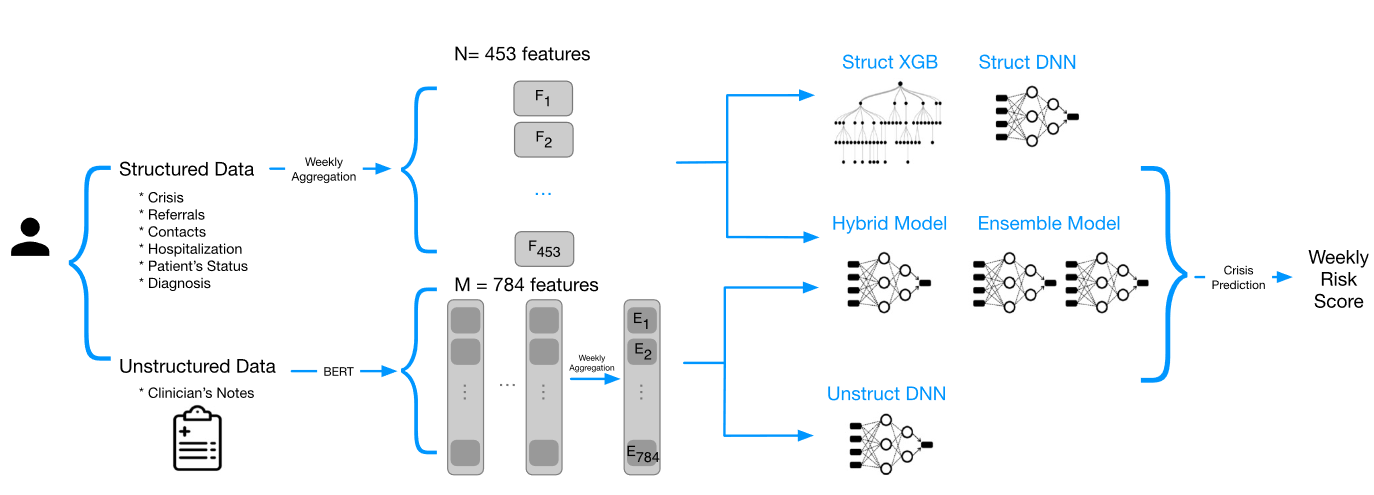
\includegraphics{images/paste-1.png}

}

\caption{\label{fig-experimentaldesign}Includes all five trained models
and the types of data used as input. Struct XGB is an XGBoost model and
the rest feed forward neural networks with ensemble DNN combining the
results of a neural network trained on structured data only and a neural
network trained on both structured and unstructured data.}

\end{figure}%

Due to the fact that relapses occur infrequently (prevalence of 1.3\%),
the models were tuned to maximize the area under the precision recall
curve (AUPRC) on the validation set which they point out is the
preferred metric for evaluationg the performance of binary
classification tasks with an unbalanced distribution.

\subsection{Performance Results}\label{performance-results}

The best model performance using only structured data was an XGBoost
model which is a tree-based classifier that implements gradient
boosting. For the model with only unstructured data and the combined
structured and unstructured data, the best model performance was a
feedforward deep neural network (DNN).

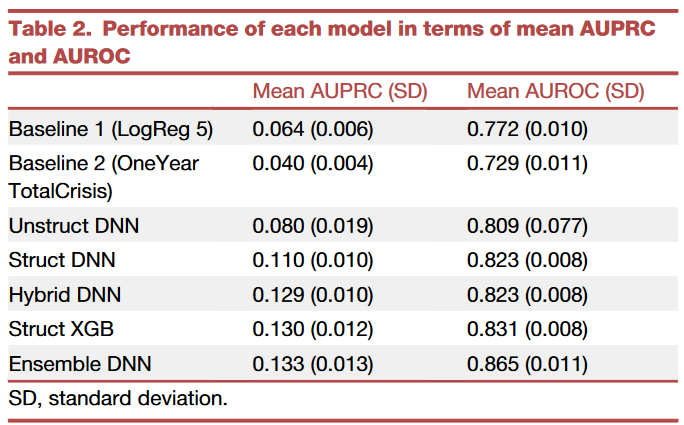
\includegraphics[width=3.64583in,height=\textheight]{images/paste-2.png}

\textbf{Provide an in-depth analysis of the performance results, and
feel free to include diagrams or data directly from the paper.}

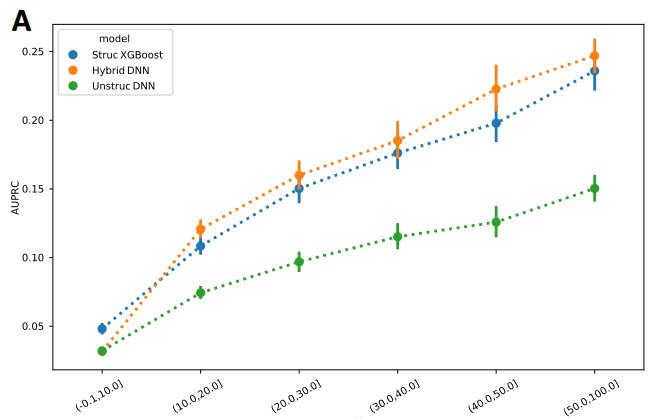
\includegraphics[width=5.34375in,height=\textheight]{images/paste-3.png}

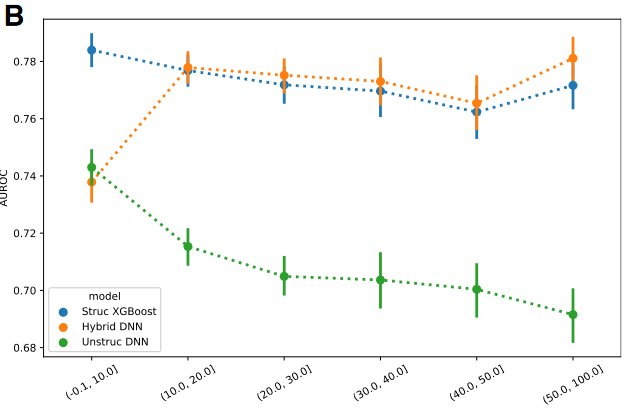
\includegraphics[width=5.34375in,height=\textheight]{images/paste-4.png}

\begin{itemize}
\tightlist
\item
  Contrast the presented solution with other existing methods, focusing
  on its advantages and disadvantages. Reflect on what we've studied in
  class, making connections where relevant.
\end{itemize}

\subsection{\texorpdfstring{\textbf{Conclusions and Further
Work:}}{Conclusions and Further Work:}}\label{conclusions-and-further-work}

\begin{itemize}
\tightlist
\item
  \textbf{Summarize the paper's key takeaways and suggest potential
  areas for future research or exploration.}
\end{itemize}

\phantomsection\label{refs}
\begin{CSLReferences}{1}{0}
\bibitem[\citeproctext]{ref-garriga2023}
Garriga, Roger, Teodora Sandra Buda, João Guerreiro, Jesús Omaña
Iglesias, Iñaki Estella Aguerri, and Aleksandar Matić. 2023.
{``Combining Clinical Notes with Structured Electronic Health Records
Enhances the Prediction of Mental Health Crises.''} \emph{Cell Reports
Medicine} 4 (11). \url{https://doi.org/10.1016/j.xcrm.2023.101260}.

\end{CSLReferences}




\end{document}
